\documentclass{article}
\usepackage[utf8]{inputenc}
\usepackage{graphicx}
\usepackage{listings}
\usepackage{xcolor}

\usepackage{amsmath}
\usepackage{centernot}

\definecolor{codegreen}{rgb}{0,0.6,0}
\definecolor{codegray}{rgb}{0.5,0.5,0.5}
\definecolor{codepurple}{rgb}{0.58,0,0.82}
\definecolor{backcolour}{rgb}{0.95,0.95,0.92}
\lstdefinestyle{mystyle}{
    backgroundcolor=\color{backcolour},   
    commentstyle=\color{codegreen},
    keywordstyle=\color{magenta},
    numberstyle=\tiny\color{codegray},
    stringstyle=\color{codepurple},
    basicstyle=\ttfamily\footnotesize,
    breakatwhitespace=false,         
    breaklines=true,                 
    captionpos=b,                    
    keepspaces=true,                 
    numbers=left,                    
    numbersep=5pt,                  
    showspaces=false,                
    showstringspaces=false,
    showtabs=false,                  
    tabsize=2
}
\lstset{style=mystyle}
\graphicspath{{./presentation_figures/}}

\title{MLPR 2019 - Assignment 2}
\author{Vasilis Gkolemis, Sokratis Lyras}

\date{October 2019}

\begin{document}

\maketitle

\section*{Question 1}

We load the data and store it in appropriate numpy arrays. We don't pass the parameter \textit{squeeze\_me=True}, because we prefer out matrices to have full shape.

\begin{lstlisting}[language = Python]
_filepath = os.path.abspath('./../../../data/ass_02/ct_data.mat')
_data = io.loadmat(_filepath)

X_train = _data['X_train']
X_val = _data['X_val']
X_test = _data['X_test']

y_train = _data['y_train']
y_val = _data['y_val']
y_test = _data['y_test']
\end{lstlisting}

\subsection*{Question 1a}

We verify that, up to numerical rounding errors, the mean of the $y\_train$ vector is zero, while this is not the case for the $y\_val$.

\begin{lstlisting}[language = Python]
np.mean(y_train) # -9.13868774539957e-15
np.mean(y_val)   # -0.2160085093241599
\end{lstlisting}


For an array $y$ we compute its mean $\tilde{\mu}$ and standard error $s$ with the following forms:

$$ \displaystyle \tilde{\mu} = \frac{1}{N} \sum_{i=1}^{N} y^{(i)} $$

$$ s = \sqrt{\frac{1}{N(N-1)} \sum_{i=1}^{N} (y^{(i)} - \tilde{\mu})^2} $$

We create a small function for implementing the above computations:

\begin{lstlisting}[language = Python]
def mean_with_sterror(x):
    m = x.mean()
    sigma = x.std(ddof = 1)
    sterror = sigma / np.sqrt(x.shape[0])
    return m, sterror
\end{lstlisting}


% The standard error $s$ of the estimation $\tilde{\mu}$ is:

% $$ s = \sqrt{VAR(\tilde{\mu})} = 
% \displaystyle \frac{\sigma}{\sqrt{N}} 
% \approx \displaystyle \frac{\tilde{\sigma}}{\sqrt{N}}$$ 

% where,

% $$ \displaystyle \tilde{\sigma}^2 = \frac{1}{N-1} \sum_{i=1}^{N} (y^{(i)} - \tilde{\mu})^2 $$


% We compute the mean with standard error of the $y\_val$ vector and of the first $N = 5785$ elements of $y\_train$ vector with the following code:

% \begin{lstlisting}[language = Python]
% def mean_with_sterror(x):
%     m = x.mean()
%     sigma = x.std(ddof = 1)
%     sterror = sigma / np.sqrt(x.shape[0])
%     return m, sterror

% m, err = mean_with_sterror(y_val)
% # m = -0.2160085093241599, err = 0.01290449880016868
% N = 5785
% m, err = mean_with_sterror(y_train[:N])
% # m = 0.01290449880016868, err = 0.011927303389170828
% \end{lstlisting}

And we apply it on $y\_val$ and the first $5785$ elements of $y\_train$:

\begin{lstlisting}[language=Python]
m, err = mean_with_sterror(y_val)
# m = -0.2160085093241599, err = 0.01290449880016868
N = 5785
m, err = mean_with_sterror(y_train[:N])
# m = -0.44247687859693674, err = 0.011927303389170828
\end{lstlisting}


We summarize the results:
\begin{itemize}
    \item $E[y_{val}] \approx - 0.216 \pm 0.013$
    \item $E[y_{test}] \approx - 0.442 \pm 0.012$ (from the first $5785$ elements)
\end{itemize}

\subsubsection*{Explanation of the misleading results}

As easily observed, the estimated mean based in the first $5785$ examples of the training set is misleading. This happens because the values are not randomly distributed inside the array.

We hold a simple experiment to show that if we randomly pick a subset of the training set, the results are as expected. We randomly sample $N = 500$ (much less than $5785$) examples from the training set and we compute their mean $\mu^{(i)}$ and standard error $s^{(i)}$. We repeat this random process $1000$ times. Finally, we compute the mean and standard deviation of the means and standard errors. 

The results, for means:

$$ \displaystyle  E[\mu] = \frac{1}{1000} \sum_{i=1}^{1000} \mu^{(i)} = -0.001 $$

$$ \displaystyle s_\mu = \sqrt{  \frac{1}{1000 - 1} \sum_{i=1}^{1000} (\mu_i - \mu_1)^2} = 0.045 $$

and for standard error:

$$ \displaystyle  E[s] = \frac{1}{1000} \sum_{i=1}^{1000} s^{(i)} = 0.045 $$

$$ \displaystyle s_s = \sqrt{  \frac{1}{1000 - 1} \sum_{i=1}^{1000} (s_i - \mu_{s})^2} = 0.001 $$

We provide the code for this small experiment:

\begin{lstlisting}[language = Python]
list_m = []
list_stderr = []
np.random.seed(2)
N = 500
y_train_tmp = copy.deepcopy(y_train)
for i in range(1000):
    np.random.shuffle(y_train_tmp)
    m, err = mean_with_sterror(y_train_tmp[:N])
    list_m.append(m)
    list_stderr.append(err)

print("Mean estimation of y_train from %d iid samples, in 1000 different executions has mean: %.3f and standard deviation: %.3f" %(N, np.mean(list_m), np.std(list_m, ddof=1)))

print("Standard error estimation of y_train from %d iid samples, in 1000 different executions has mean: %.3f and standard deviation: %.3f" %(N, np.mean(list_stderr), np.std(list_stderr, ddof = 1)))
\end{lstlisting}

\subsection*{Question 1b}

We use python, so our indices are zero-based. 
The code for identifying constant features:
\begin{lstlisting}[language = Python]
threshold = 10e-10
ind_const_features = np.where(X_train.var(0) <= threshold)[0]
# array([ 59,  69, 179, 189, 351])
\end{lstlisting}
Constant columns are: $\{59,  69, 179, 189, 351\}$


The code for identifying duplicates:
\begin{lstlisting}[language = Python]
duplicates = []
for j in range(X_train.shape[1]):
    f1 = X_train[:,j]
    tmp = X_train[:, j+1:] - np.expand_dims(f1, -1)
    indices = np.where((np.var(tmp, 0) <= threshold))[0] + j + 1
    duplicates.append(indices)

ind_duplicate_features = np.concatenate(duplicates).ravel()
ind_duplicate_features = np.sort(np.unique(ind_duplicate_features))
# array([ 69,  78,  79, 179, 188, 189, 199, 287, 351, 359])
\end{lstlisting}

Duplicates \textbf{later} columns are: $ {69,  78,  79, 179, 188, 189, 199, 287, 351, 359} $


\section*{Question 2}

We create a function that fits the learnable parameters to the data. Firstly, we create an augmented version of X matrix:

$$ \displaystyle
X_{aug} = \begin{vmatrix}
    X_{train} & \textbf{1} \\
    \sqrt{a}I_D & \textbf{0} 
\end{vmatrix}
$$

Afterwards we use np.linalg.lstsq routine to compute the optimal parameters $\textbf{w}, b$. This is done inside the following function:

\begin{lstlisting}[language= Python]
def fit_linreg(X, yy, alpha):
    # data augmentation
    D = X.shape[1]
    N = X.shape[0]
    
    reg = np.sqrt(alpha) * np.eye(D, D)
    X1 = np.concatenate( (X, np.ones((N, 1)) ), axis = 1)
    reg1 = np.concatenate( (reg, np.zeros((reg.shape[1], 1)) ), axis = 1)
    X_aug = np.concatenate( (X1, reg1), axis=0)
    y_aug = np.concatenate( (yy, np.zeros((D, 1))), axis = 0)

    # lstsq
    W, SSE, rank, singulars = np.linalg.lstsq(X_aug, y_aug, rcond=None)
    W_lstsq = W[:-1]
    b_lstsq = W[-1]
    return W_lstsq, b_lstsq
\end{lstlisting}

We fit the model to the data using two different approaches:
\begin{itemize}
    \item our method (fit\_linreg) 
    \item fit\_linreg\_gradopt, which is provided on the package ct\_support\_code
\end{itemize}

\begin{lstlisting}[language= Python]
# least square method
W_lstsq, b_lstsq = fit_linreg(X_train, y_train, 10)

# gradient method
alpha = 10
W_grad, b_grad = fit_linreg_gradopt(X_train, np.squeeze(y_train), alpha)
\end{lstlisting}

We compute the RMSE in both cases with the following code:

\begin{lstlisting}[language= Python]
def compute_RMSE(X, y, w, b):
    # expand_dims to all single dimensional arrays
    if len(y.shape) == 1:
        y = np.expand_dims(y, -1)

    if len(w.shape) == 1:
        w = np.expand_dims(w, -1)
    
    # compute RMSE
    y_bar = np.dot(X, w) + b
    square_erros = np.square(y_bar - y)
    RMSE = np.sqrt(np.mean(square_erros))
    return RMSE 

RMSE_lstsq_tr = compute_RMSE(X_train, y_train, W_lstsq, b_lstsq)
RMSE_lstsq_val = compute_RMSE(X_val, y_val, W_lstsq, b_lstsq)

RMSE_grad_tr = compute_RMSE(X_train, y_train, W_grad, b_grad)
RMSE_grad_val = compute_RMSE(X_val, y_val, W_grad, b_grad)
\end{lstlisting}

We report the RMSE in both cases:

\begin{center}
\begin{tabular}{ | c | c | c | } 
\hline
 & Training & Validation \\
\hline
Least Squares & 0.35575 & 0.42059 \\ 
\hline
Gradient & 0.35576 & 0.42061 \\ 
\hline
\end{tabular}
\end{center}

We observe that the two RMSE are very close, but not identical. The gradient based optimization method cannot ensure that it will find the exact optimal, but because our cost function is convex it must converge to the optimal value. So the results are as expected.


\section*{Question 3}

\subsection*{Question 3a}

We use the the provided \textit{random\_proj} routine to create the projection matrix. We create the following function for projecting the input, fitting the projected data and computing the RMSE:

\begin{lstlisting}[language=Python]
def fit_and_measure_on_projection(K):
    alpha = 10
    proj_mat = random_proj(D, K)

    # projected X
    X_train_proj = np.dot(X_train, proj_mat)
    X_val_proj = np.dot(X_val, proj_mat)

    results = {"K": K}

    # fitting
    W_lstsq_proj, b_lstsq_proj = fit_linreg(X_train_proj, y_train, alpha)

    # RMSE
    results['RMSE_lstsq_tr'] = compute_RMSE(X_train_proj, y_train, W_lstsq_proj, b_lstsq_proj)
    results['RMSE_lstsq_val'] = compute_RMSE(X_val_proj, y_val, W_lstsq_proj, b_lstsq_proj)
    
    return results

K = 10
q3a_results_proj_10 = fit_and_measure_on_projection(K)

K = 100
q3a_results_proj_100 = fit_and_measure_on_projection(K)
\end{lstlisting}


The errors we obtained are the following:
\begin{center}
\begin{tabular}{ | c | c | c | }
\hline
\multicolumn{3}{|c|}{ K = 10 } \\
\hline
 & Training & Validation \\
\hline
Least Squares & 0.76299 & 0.80863\\ 
\hline

\hline 
\hline

\multicolumn{3}{|c|}{ K = 100 } \\
\hline
 & Training & Validation \\
\hline
Least Squares & 0.47499 & 0.50218 \\ 
\hline
\end{tabular}
\end{center}


As we reduce the dimensionality, the new training error must be larger or equal than before. Since our input matrix $X\_train$ is full rank (as we checked), every feature gives information, so reducing the dimensionality leads to strictly higher error.


\subsection*{Question 3b}

It is clear that a very big fraction of feature 46 is either $0$ or $-0.25$. More specifically, in the whole training set almost $80.36\%$ of the examples are either $0$ or $-0.25$.

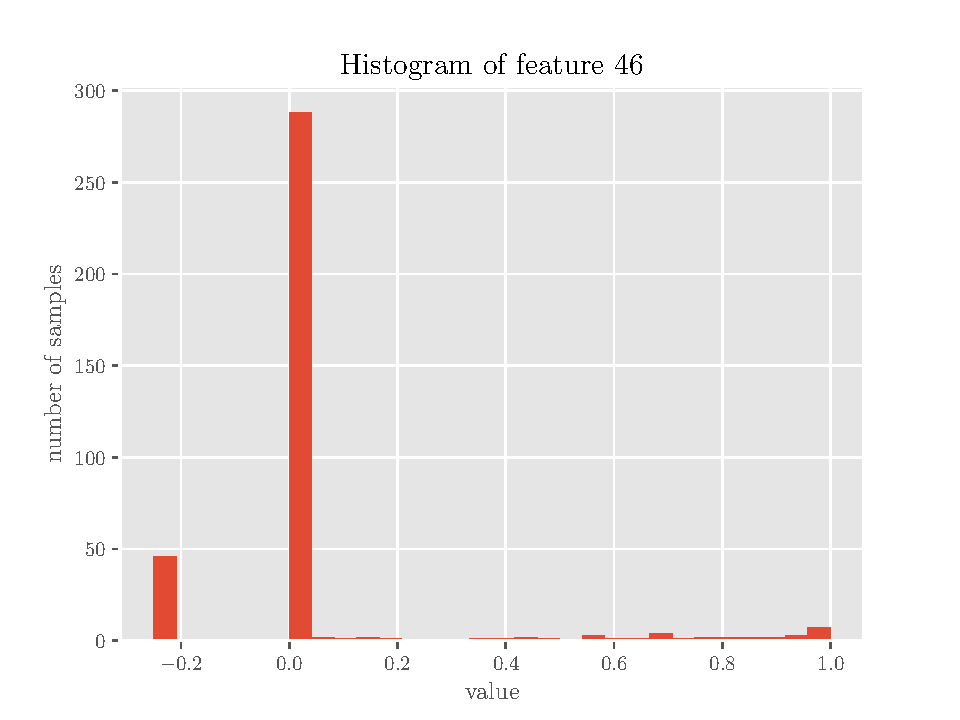
\includegraphics[scale=0.75]{fig_01.pdf}


We create a function for fitting the augmented data and measuring the RMSE:

\begin{lstlisting}[language=Python]
def fit_and_measure_added_binaries():
    alpha = 10

    # projected X
    def aug_fn(X): return np.concatenate([X, X == 0, X < 0], axis=1)

    X_train_aug = aug_fn(X_train)
    X_val_aug = aug_fn(X_val)

    # fitting
    W_lstsq, b_lstsq = fit_linreg(X_train_aug, y_train, alpha)
    
    # RMSE
    results = {}
    results['RMSE_lstsq_tr'] = compute_RMSE(X_train_aug, y_train, W_lstsq, b_lstsq)
    results['RMSE_lstsq_val'] = compute_RMSE(X_val_aug, y_val, W_lstsq, b_lstsq)
    
    return results

q3b_results_added_binaries = fit_and_measure_added_binaries()
\end{lstlisting}

We report the results:

\begin{center}
\begin{tabular}{ | c | c | c | }
\hline
 & Training & Validation \\
\hline
RMSE & 0.31783 & 0.37698 \\ 
\hline
\end{tabular}
\end{center}

The training error has improved. This is expected, as the augmented X matrix:
\begin{itemize}
    \item contains the initial $X\_train$ as a part of it
    \item has more features than $X\_train$
    \item has higher rank than $X\_train$ $(=831)$
    
\end{itemize}
We also notice that the validation error has been improved as well. This is a much stronger indicator that this type of augmentation, is beneficial in terms of accuracy.


\section*{Question 4}

We fit each separate logistic regression model and store each parameters in a dictionary, with the following code:

\begin{lstlisting}[language=Python]
# number of separate classification tasks
K = 10 

# compute intervals
mx = np.max(y_train)
mn = np.min(y_train)
hh = (mx-mn)/(K+1)
thresholds = np.linspace(mn+hh, mx-hh, num=K, endpoint=True)

# set regularizer
alpha = 10 

# init dict to store parameters
weight_dict = {}

# fit for each interval
for kk in range(K):
    # set labels
    labels = y_train > thresholds[kk]

    # fit logistic regression
    ww, bb = fit_logreg_gradopt(X_train, np.squeeze(labels), alpha)
    
    # store weights
    weight_dict[kk] = {}
    weight_dict[kk]['w'] = ww
    weight_dict[kk]['b'] = bb
\end{lstlisting}

We stack the learned parameters into a matrix:

\begin{lstlisting}[language=Python]
weights = []
bias = []
for key, value in weight_dict.items():
    weights.append(value["w"])
    bias.append(value["b"])
ww = np.stack(weights, axis=1)
bb = np.expand_dims(np.stack(bias), 0)
\end{lstlisting}

We also define the sigmoid and project initial matrices to new dimension. We name the projected matrices with the suffix "\_smart":

\begin{lstlisting}[language=Python]
def sigmoid(x): return 1/ (1 + np.exp(-x))
X_train_smart = sigmoid(np.dot(X_train, ww) + bb)
X_val_smart = sigmoid(np.dot(X_val, ww) + bb)
X_test_smart = sigmoid(np.dot(X_test, ww) + bb)
\end{lstlisting}

Finally, we fit the projected inputs to a linear regression model and compute the appropriate RMSE:

\begin{lstlisting}[language=Python]
# fit linear regression
alpha = 10
W_smart, b_smart = fit_linreg(X_train_smart, y_train, alpha)

# compute errors
q4_RMSE_smart_tr = compute_RMSE(X_train_smart, y_train, W_smart, b_smart)
q4_RMSE_smart_val = compute_RMSE(X_val_smart, y_val, W_smart, b_smart)
\end{lstlisting}

We report the results:

\begin{center}
\begin{tabular}{ | c | c | c | }
\hline
 & Training & Validation \\
\hline
RMSE & 0.13825 & 0.25213 \\ 
\hline
\end{tabular}
\end{center}

We observe a massive improvement in the training and validation error. Adding a non-linear projection unit before the final linear regression, has made our predictions more accurate. (Even more than the linear regression models operating in the augmented X matrix). By fitting the 10 logistic regression models, we managed to create a learned non-linear projection mechanism, that maintains more information that the random projection matrix.

\section*{Question 5}

We fit two Neural Networks with the exact same architecture and different initializations.

\begin{lstlisting}[language=Python]
# random initialization
init_params = (np.random.randn(10), np.array(0), np.random.randn(10, D), np.zeros(10))
ww1, bb1, V1, bk1 = fit_cnn_gradopt(X_train, np.squeeze(y_train), 10)
params1 = (ww1, bb1, V1, bk1)

# sophisticated initialization
init_params = (np.squeeze(W_smart), np.squeeze(b_smart), ww.T, np.squeeze(bb))
ww2, bb2, V2, bk2 = fit_cnn_gradopt(X_train, np.squeeze(y_train), 10, init_params)
params2 = (ww2, bb2, V2, bk2)
\end{lstlisting}

We then compute the RMSE for each case:

\begin{lstlisting}[language=Python]
def compute_RMSE_cnn(X, y, params):
    y_bar = np.expand_dims(nn_cost(params, X), -1)
    square_error = np.square(y_bar - y)
    RMSE = np.sqrt(np.mean(square_error))
    return RMSE

q5_RMSE_rand_tr = compute_RMSE_cnn(X_train, y_train, params1)
q5_RMSE_rand_val = compute_RMSE_cnn(X_val, y_val, params1)

q5_RMSE_soph_tr = compute_RMSE_cnn(X_train, y_train, params2)
q5_RMSE_soph_val = compute_RMSE_cnn(X_val, y_val, params2)
\end{lstlisting}

\begin{center}
\begin{tabular}{ | c | c | c | }
\hline
 & Training & Validation \\
\hline
Random Init & 0.09660 & 0.25868 \\ 
\hline
Sophisticated Init & 0.10435 & 0.25692 \\ 
\hline
\end{tabular}
\end{center}

In the random initialization, we initialize the weights of the matrices from a normal distribution and the biases with zero.
As we can see, both methods produce almost the same results. This means that the number of learnable parameters of the cnn is relatively small for the dimensionality of the problem and and the amount of training data is large enough. Thus, a good local optima can easily be reached from a random initial point.

We also observe that the RMSE of the validation set of the model in question 4, is approximately the same with the RMSE of the neural network. Hence, neural network could not learn anything more than the previous model. 


\section*{Question 6}

In this section, we thought of not creating a new model from scratch, but taking advantage of the work we have done so far. Thus we tried various ideas that could fit to the already implemented framework, including PCA, different weight initialization, input normalization etc. We observed that the most effective methods, in terms of the validation error, are:

\begin{itemize}
    \item Add gaussian noise with to the training data $X\_train + \mathcal{N}(0,\sigma^2)$
    \item Change the units of the hidden layer
    \item Augment the input matrix $X\_train$ with the binary features of Question $3$
\end{itemize}\\

The initiatives for testing these ideas was the overfiting we observed in the previous Neural Network models. That is why we added Gaussian noise to the inputs. We also though of experimenting with adding binaries, because of the accuracy increase we observed in question 3. Finally, we tested the increasing the units of the hidden layers. This idea intially conflicts with the observed overfiting, but in combination with adding Gaussian noise, it helps our network to learn more complex representations.

We held an experiment trying all the possible combination of the hyperparameters \\ $$(\sigma, K, \text{adding\_binaries}) \in \{0.3, 0.4, 0.45, 0.5, 0.55, 0.6\}\times \{10, 20, 40, 60\}\times \{True, False\}$$

For each combination of the above hyperparameters, we run the training process $5$ times (independently) and we computed the mean validation error of the $5$ executions and the standard error. Since adding Gaussian Noise and using Random Initialization of the weights make the whole process random, this repetition helps us check the statistical significance of the different errors.

We present the results in the Figure \ref{fig:val_error}:

\begin{figure}[h]
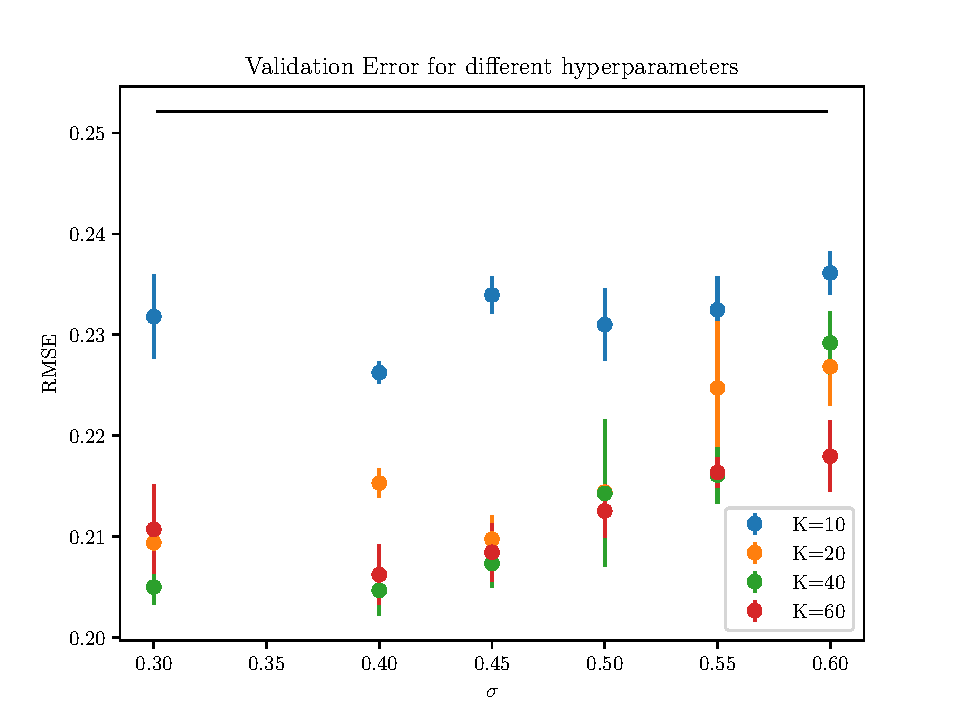
\includegraphics[scale=0.8]{val_error.pdf}
\caption{The black horizontal line on the top, shows the validation error of the best model of the previous questions. The error bars show the standard error of the mean RMSE across the $5$ executions. We observe high overlapping so we cannot easily decide which model is the best, but we can safely suggest the the model with $(s=0.4, K=40, \text{add\_binaries=False})$ show a significant improvement in terms of validation error from the models we had obtained so far.}
\centering
\label{fig:val_error}
\end{figure}


The best model in terms of mean RMSE along the 5 different executions has hyperparameters $(\sigma=0.4, K=40, \text{add\_binaries=False})$ and mean validation RMSE = $0.205$ with standard error $0.0025$.

This model has a generalisation RMSE in the test set $0.239$ with standard error $0.002$.


We provide the code used for holding this experiment:

\begin{lstlisting}[language=Python]
def fit_and_RMSE_cnn(s, k, add_binaries, inputs):
    def aug_fn(X): return np.concatenate([X, X == 0, X < 0], axis=1)

    X_train = inputs['X_train']
    X_val = inputs['X_val']
    X_test = inputs['X_test']
    y_train = inputs['y_train']
    y_val = inputs['y_val']
    y_test = inputs['y_test']
    D = X_train.shape[1]

    alpha = 10
    if add_binaries:
        X_train = aug_fn(X_train)
        X_val = aug_fn(X_val)
        X_test = aug_fn(X_test)
        D = 3*D

    init_params = (np.random.randn(k), np.array(0), np.random.randn(k, D), np.zeros(k))
    ww1, bb1, V1, bk1 = fit_cnn_gradopt(X_train + np.random.standard_normal(X_train.shape) * s,
                                        np.squeeze(y_train), alpha, init_params)

    params = (ww1, bb1, V1, bk1)

    results = {}
    results['RMSE_tr'] = compute_RMSE_cnn(X_train, y_train, params)
    results['RMSE_val'] = compute_RMSE_cnn(X_val, y_val, params)
    results['RMSE_test'] = compute_RMSE_cnn(X_test, y_test, params)
    return results, params

sig = [0.3, 0.4, 0.45, 0.5, 0.55, 0.6]
K = [10, 20, 40, 60]
add_binaries = [True, False]
inputs = {'X_train': X_train,
          'X_val': X_val,
          'X_test': X_test,
          'y_train': y_train,
          'y_val': y_val,
          'y_test': y_test}

results = []
params = []
hyperparams = []
for ii, s in enumerate(sig):
    results.append([])
    params.append([])
    hyperparams.append([])
    for jj, k in enumerate(K):
        results[ii].append([])
        params[ii].append([])
        hyperparams[ii].append([])
        for kk, bin in enumerate(add_binaries):
            results[ii][jj].append([])
            params[ii][jj].append([])
            hyperparams[ii][jj].append([])
            for n in range(5):
                tmp = fit_and_RMSE_cnn(s,k,bin,inputs)
                results[ii][jj][kk].append(tmp[0])
                params[ii][jj][kk].append(tmp[1])
                hyperparams[ii][jj][kk].append({'s':s, 'k':k, 'add_binaries':bin, 'n':n})

\end{lstlisting}






\end{document}
